%\documentclass[11pt]{paper}
%\usepackage{palatino}
%\usepackage{amsfonts,amsmath,amssymb}
%% \usepackage{graphicx}
%
%\usepackage{listings}
%\usepackage{textcomp}
%\usepackage{color}
%
%\definecolor{dkgreen}{rgb}{0,0.6,0}
%\definecolor{gray}{rgb}{0.5,0.5,0.5}
%\definecolor{mauve}{rgb}{0.58,0,0.82}
%
%\lstset{frame=tb,
%  language=R,
%  aboveskip=3mm,
%  belowskip=3mm,
%  showstringspaces=false,
%  columns=flexible,
%  basicstyle={\small\ttfamily},
%  numbers=none,
%  numberstyle=\tiny\color{gray},
%  keywordstyle=\color{blue},
%  commentstyle=\color{dkgreen},
%  stringstyle=\color{mauve},
%  breaklines=true,
%  breakatwhitespace=true,
%  tabsize=3
%}
%
%
%
%\ifx\pdftexversion\undefined
%    \usepackage[dvips]{graphicx}
%\else
%    \usepackage[pdftex]{graphicx}
%    \usepackage{epstopdf}
%    \epstopdfsetup{suffix=}
%\fi
%
%\usepackage{subfig}
%
%
%% This allows pdflatex to print the curly quotes in the
%% significance codes in the output of the GAM.
%\UseRawInputEncoding
%
%\begin{document}
%
%%%%%%%%%%%%%%%%%%%%%%%%%%%%%%%%%%%%%%%%%
%% Problem Set 8
%%%%%%%%%%%%%%%%%%%%%%%%%%%%%%%%%%%%%%%%%
%
%\pagestyle{empty}
%{\noindent\bf Spring 2023 \hfill Brandon~Parmanand}
%\vskip 16pt
%\centerline{\bf University of Central Florida}
%\centerline{\bf College of Business}
%\vskip 16pt
%\centerline{\bf QMB 6911}
%\centerline{\bf Capstone Project in Business Analytics}
%\vskip 10pt
%\centerline{\bf Solutions:  Problem Set \#8}
%\vskip 32pt
%\noindent
%% 
%
%
%{\color{red} 
%Quick comments:
%Excellent work; no major problems with modeling decisions.
%Each of you made different decisions with respect to model specification
%and built models of similar accuracy.
%The implementation of FWL regressions and nonparametric/semiparametric models was well done.
%
%The only part that I did not find was a comparison of the GAM vs. the Box-Tidwell modeling framework (please correct me if I am wrong). Other than that minor misstep, this was great.
%}
%
%\section{Data Description}
%
%This analysis follows the script \texttt{PS8.R} to produce a more accurate model for used tractor prices with the data from \texttt{HomeSales.dat} in the \texttt{Data} folder. 
I will revisit the recommended linear model,
which included a Box Tildwell specification for age. 
I will investigate this nonlinear relationship
by incorporating a nonparametric specification
for the value of age. 
Similarly, for the other continuous variables Lot Size and Transit Score, 
to investigate whether these forms of depreciation
are best described with nonlinear forms. 


%%%%%%%%%%%%%%%%%%%%%%%%%%%%%%%%%%%%%%%%
\clearpage
\section{Linear Regression Model}
%%%%%%%%%%%%%%%%%%%%%%%%%%%%%%%%%%%%%%%%

 

\subsection{Box Tildwell Specification for Age}

% 

\begin{table}
\begin{center}
\begin{tabular}{l c}
\hline
 & Model 1 \\
\hline
(Intercept)       & $12.27956^{***}$ \\
                  & $(0.03468)$      \\
TypeOfBuyerRental & $0.11437^{***}$  \\
                  & $(0.01590)$      \\
Age               & $-0.03428^{***}$ \\
                  & $(0.00365)$      \\
NumBeds2          & $0.22090^{***}$  \\
                  & $(0.02576)$      \\
NumBeds3          & $0.41973^{***}$  \\
                  & $(0.03114)$      \\
NumBeds4          & $0.60678^{***}$  \\
                  & $(0.03437)$      \\
NumBeds6          & $0.69817^{***}$  \\
                  & $(0.05573)$      \\
NumBeds8          & $1.07728^{***}$  \\
                  & $(0.06068)$      \\
NumBaths2         & $0.07219^{***}$  \\
                  & $(0.01376)$      \\
NumBaths3         & $0.10791^{***}$  \\
                  & $(0.02694)$      \\
LotSize           & $0.00004^{***}$  \\
                  & $(0.00000)$      \\
HasGarage         & $0.26785^{***}$  \\
                  & $(0.01924)$      \\
HasSecGate        & $0.22254^{***}$  \\
                  & $(0.01788)$      \\
TransitScore      & $0.06332^{***}$  \\
                  & $(0.00296)$      \\
bt\_age\_log\_age & $0.00608^{***}$  \\
                  & $(0.00094)$      \\
\hline
R$^2$             & $0.67999$        \\
Adj. R$^2$        & $0.67817$        \\
Num. obs.         & $2473$           \\
\hline
\multicolumn{2}{l}{\scriptsize{$^{***}p<0.001$; $^{**}p<0.01$; $^{*}p<0.05$}}
\end{tabular}
\caption{Age BT Model for Home Prices}
\label{tab:reg_bt_age}
\end{center}
\end{table}

% 

The results of this regression specification are shown in 
Table \ref{tab:reg_bt_age}. 
The BT Age variable has a coefficient of 
% $6.082e-03$,
$6.082\times10^{-3}$,  
which is larger than the standard error of 
% $9.404e-03$, 
$9.404\times10^{-3}$, 
which is evidence against the null hypothesis of a positive or zero coefficient. 
I conclude that the log of the sale price does decline for older homes. 


%	With the squared horsepower variable, the $\bar{R}^2$ is $0.6503$, indicating that it is a slightly stronger model than the others we considered. 
%	The $F$-statistic is large, indicating that it is a better candidate than the simple average log sale price. 
%	The new BT age variable is statistically significant and the theory behind it is sound, since above a certain point. 
%	This new model is improved over the previous models with other specifications for age.
Next, I will attempt to improve on this specification. 





%%%%%%%%%%%%%%%%%%%%%%%%%%%%%%%%%%%%%%%%
\clearpage
\section{Nonlinear Specifications}
%%%%%%%%%%%%%%%%%%%%%%%%%%%%%%%%%%%%%%%%


% \clearpage
\subsection{Nonparametric Specification for Age}


The specification in 
Table \ref{tab:reg_bt_age}
assumes a Box Tildwell form for
the relationship between price and age. 
To consider the age variable alone, 
while accounting for the effects of other variables, 
one can fit a nonparametric model to the residuals 
from a model of house prices, 
after regressing house prices on the other variables. 
This leaves only the variation in house prices that is not explained by the other variables. 
Going one step further, perform the same transformation to the age variable:
take the residuals from a model of age, 
after regressing age on the other variables. 
This allows a model that would fit exactly the same as if it were estimated within a full model with all variables included. 

The models shown in
Table \ref{tab:reg_bt_age_fwl}
illustrate this possibility. 
Model 1 is the original model in 
Table \ref{tab:reg_bt_age}. 
Model 2 is a regression omitting the age variables. 
Model 3 is a regression to predict age with the other explanatory variables in Model 2.
Model 4 is a regression to predict BT age with the other explanatory variables in Model 2.
Finally, Model 5 shows the coefficients for age
from a regression of the residuals of Model 2
on the residuals from Model 3. 
Notice that these coefficients match those in Model 1. 
You might notice a slight difference in the standard errors, however, 
because these are calculated assuming coefficients 
for two variables, age and BT age,
rather than the full suite of ten parameters.
This equivalence of the coefficients can be used to fit
nonlinear models between a pair of variables by 
partialing out the effect of the other variables.


\begin{table}
\begin{center}
\begin{footnotesize}
\begin{tabular}{l c c c c c}
\hline
 & Original (1) & Reduced (2) & Age (3) & Age. BT. (4) & FWL Age (5) \\
\hline
(Intercept)       & $12.27956^{***}$ & $12.09348^{***}$ & $10.82068^{***}$ & $30.40148^{***}$ &                  \\
                  & $(0.03468)$      & $(0.03722)$      & $(1.59294)$      & $(6.17785)$      &                  \\
TypeOfBuyerRental & $0.11437^{***}$  & $0.05066^{**}$   & $5.70467^{***}$  & $21.68169^{***}$ &                  \\
                  & $(0.01590)$      & $(0.01789)$      & $(0.76573)$      & $(2.96969)$      &                  \\
Age               & $-0.03428^{***}$ &                  &                  &                  &                  \\
                  & $(0.00365)$      &                  &                  &                  &                  \\
NumBeds2          & $0.22090^{***}$  & $0.21786^{***}$  & $0.27924$        & $1.07401$        &                  \\
                  & $(0.02576)$      & $(0.02932)$      & $(1.25470)$      & $(4.86603)$      &                  \\
NumBeds3          & $0.41973^{***}$  & $0.41369^{***}$  & $0.62368$        & $2.52189$        &                  \\
                  & $(0.03114)$      & $(0.03544)$      & $(1.51679)$      & $(5.88251)$      &                  \\
NumBeds4          & $0.60678^{***}$  & $0.61552^{***}$  & $-0.45182$       & $-1.11001$       &                  \\
                  & $(0.03437)$      & $(0.03911)$      & $(1.67365)$      & $(6.49083)$      &                  \\
NumBeds6          & $0.69817^{***}$  & $0.71277^{***}$  & $-0.81578$       & $-2.19939$       &                  \\
                  & $(0.05573)$      & $(0.06342)$      & $(2.71421)$      & $(10.52639)$     &                  \\
NumBeds8          & $1.07728^{***}$  & $1.12632^{***}$  & $-4.32464$       & $-16.31485$      &                  \\
                  & $(0.06068)$      & $(0.06903)$      & $(2.95412)$      & $(11.45684)$     &                  \\
NumBaths2         & $0.07219^{***}$  & $0.07575^{***}$  & $-0.34009$       & $-1.33279$       &                  \\
                  & $(0.01376)$      & $(0.01566)$      & $(0.66996)$      & $(2.59826)$      &                  \\
NumBaths3         & $0.10791^{***}$  & $0.11104^{***}$  & $-0.71642$       & $-3.52346$       &                  \\
                  & $(0.02694)$      & $(0.03064)$      & $(1.31142)$      & $(5.08601)$      &                  \\
LotSize           & $0.00004^{***}$  & $0.00004^{***}$  & $-0.00012$       & $-0.00046$       &                  \\
                  & $(0.00000)$      & $(0.00000)$      & $(0.00018)$      & $(0.00069)$      &                  \\
HasGarage         & $0.26785^{***}$  & $0.21408^{***}$  & $4.58242^{***}$  & $16.98939^{***}$ &                  \\
                  & $(0.01924)$      & $(0.02178)$      & $(0.93185)$      & $(3.61395)$      &                  \\
HasSecGate        & $0.22254^{***}$  & $0.19835^{***}$  & $2.34684^{**}$   & $9.25280^{**}$   &                  \\
                  & $(0.01788)$      & $(0.02032)$      & $(0.86937)$      & $(3.37163)$      &                  \\
TransitScore      & $0.06332^{***}$  & $0.06732^{***}$  & $-0.34281^{*}$   & $-1.27462^{*}$   &                  \\
                  & $(0.00296)$      & $(0.00336)$      & $(0.14398)$      & $(0.55840)$      &                  \\
bt\_age\_log\_age & $0.00608^{***}$  &                  &                  &                  &                  \\
                  & $(0.00094)$      &                  &                  &                  &                  \\
age\_resid        &                  &                  &                  &                  & $-0.03428^{***}$ \\
                  &                  &                  &                  &                  & $(0.00364)$      \\
age\_2\_resid     &                  &                  &                  &                  & $0.00608^{***}$  \\
                  &                  &                  &                  &                  & $(0.00094)$      \\
\hline
R$^2$             & $0.67999$        & $0.58512$        & $0.02593$        & $0.02498$        & $0.22867$        \\
Adj. R$^2$        & $0.67817$        & $0.58310$        & $0.02118$        & $0.02023$        & $0.22804$        \\
Num. obs.         & $2473$           & $2473$           & $2473$           & $2473$           & $2473$           \\
\hline
\multicolumn{6}{l}{\tiny{$^{***}p<0.001$; $^{**}p<0.01$; $^{*}p<0.05$}}
\end{tabular}
\end{footnotesize}
\caption{BT Model for House Prices: FWL Regressions}
\label{tab:reg_bt_age_fwl}
\end{center}
\end{table}


\pagebreak 
To illustrate the fit of the model, 
Figure \ref{fig:dev_vs_age} shows a scatter plot 
of the residual log prices on age. 
The observations are shown in blue
and the fitted values are shown in red.
The variation in the fitted values results from the 
fact that it is not plotted against the transformed excess age variable used in the regressions.


\begin{figure}[h!]
  \centering
  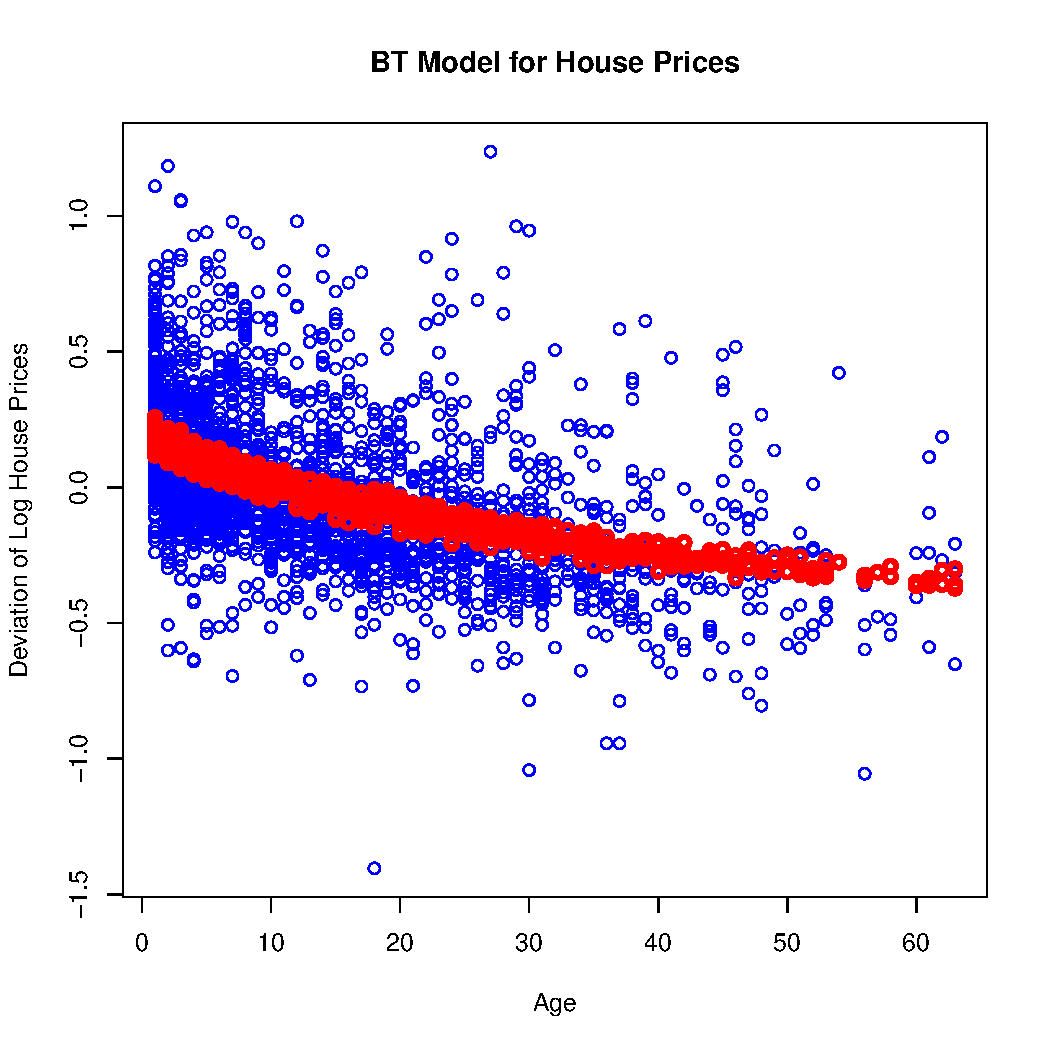
\includegraphics[scale = 0.5, keepaspectratio=true]{../Figures/dev_vs_age}
  \caption{Linear-Box Tildwell Model for House Prices} \label{fig:dev_vs_age}
\end{figure}



\pagebreak
As a comparison, Figure \ref{fig:dev_vs_age_dev} 
augments the above by showing the plot against the 
residuals from the regression for age:
the ``excess age'' compared to what would be 
expected given the other characteristics of a house.


\begin{figure}[h!]
  \centering
  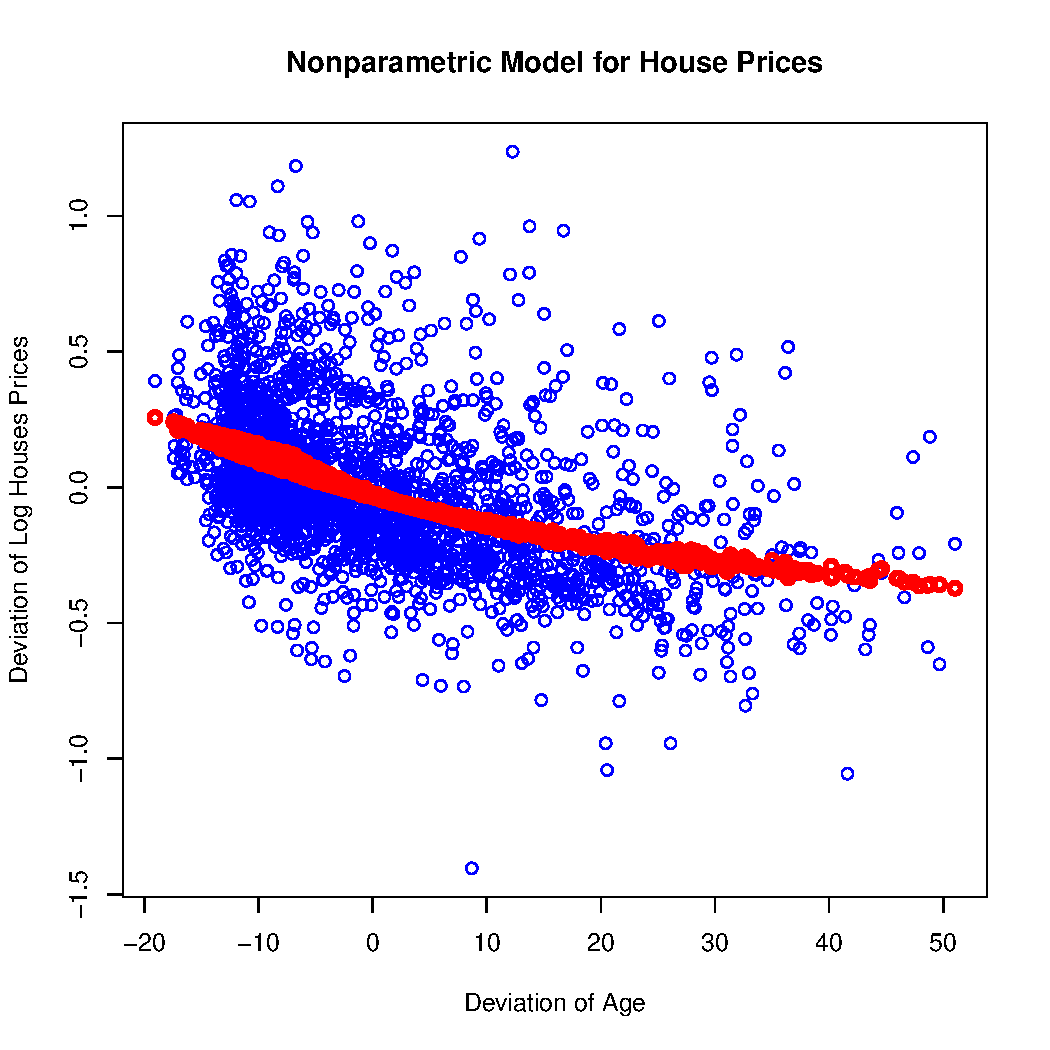
\includegraphics[scale = 0.5, keepaspectratio=true]{../Figures/dev_vs_age_dev}
  \caption{Linear-BT Model for House Prices: Excess Age} \label{fig:dev_vs_age_dev}
\end{figure}

\clearpage
Now consider a nonparametric specification for 
the relationship between prices and age.
Figure \ref{fig:dev_np_vs_age_dev} 
overlays the nonparametric estimate (shown in green) with the above in 
Figure \ref{fig:dev_vs_age_dev}.
The pattern has more variation in slope but 
closely follows the prediction from the BT model. 
So far, it appears that the BT form
is close enough.

\begin{figure}[h!]
  \centering
  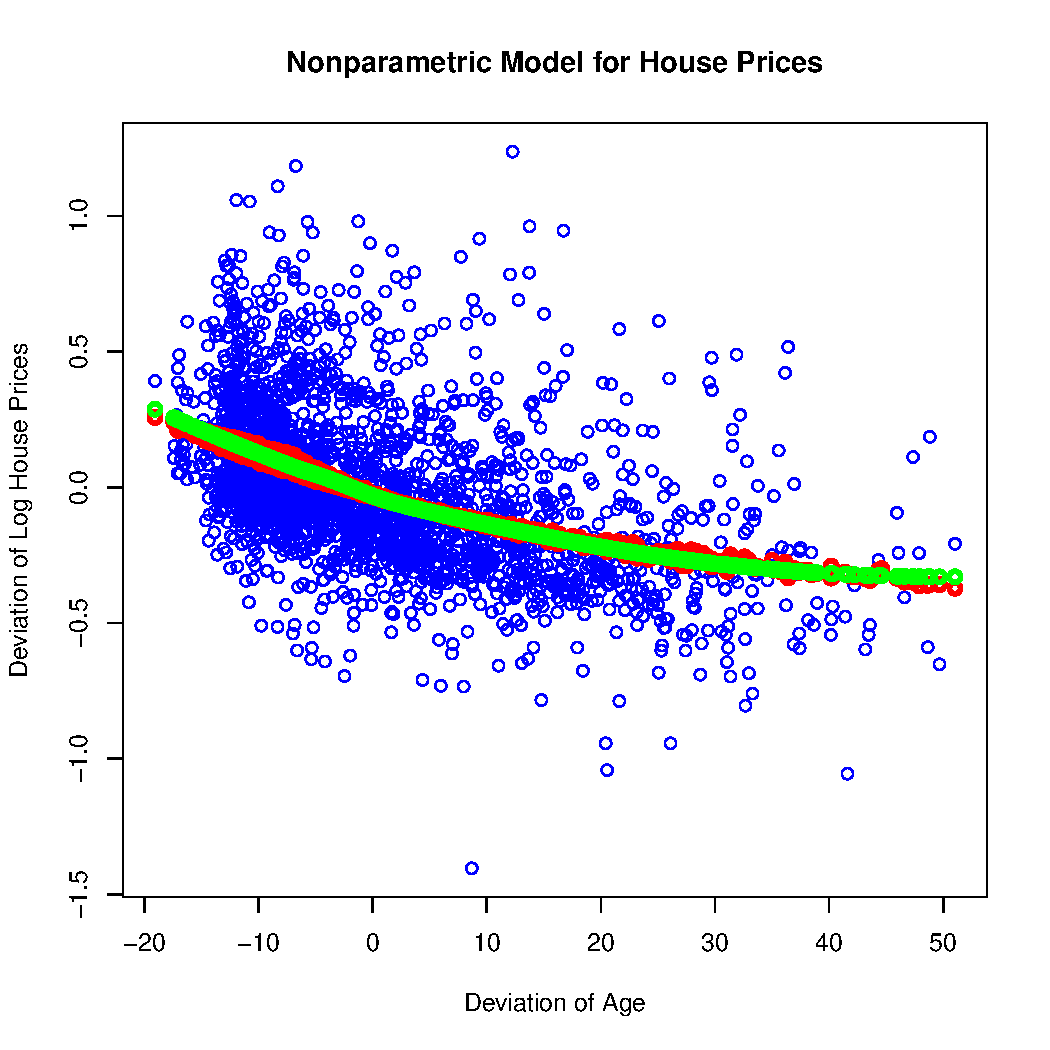
\includegraphics[scale = 0.5, keepaspectratio=true]{../Figures/dev_np_vs_age_dev}
  \caption{Nonparametric Model for House Prices: Excess Age} \label{fig:dev_np_vs_age_dev}
\end{figure}

 

\clearpage
Finally, consider a set of nonparametric specifications for 
the relationship between prices and age.
Figure \ref{fig:dev_np_vs_age_dev_bw} 
overlays other nonparametric estimates with the above in 
Figure \ref{fig:dev_np_vs_age_dev}.
The points in orange and in magenta represent
alternate models with different degrees of smoothing. 
%
When we estimated probability densities,
we adjusted the bandwidth parameter to fit
with different degrees of smoothness.
The \texttt{loess} method used for the nonparametric method has a span parameter for this function.
The default smoother \texttt{span} (bandwidth parameter) is 0.75.

In the magenta points, with \texttt{span} parameter 0.1, the pattern has more variation in slope but 
closely follows the prediction from the BT model. 
The smoother curve in orange 
even more closely represents a straight line. 
Again, it appears that the BT form
is close enough.
Perhaps the result will be different for other continuous variables in the model.

\begin{figure}[h!]
  \centering
  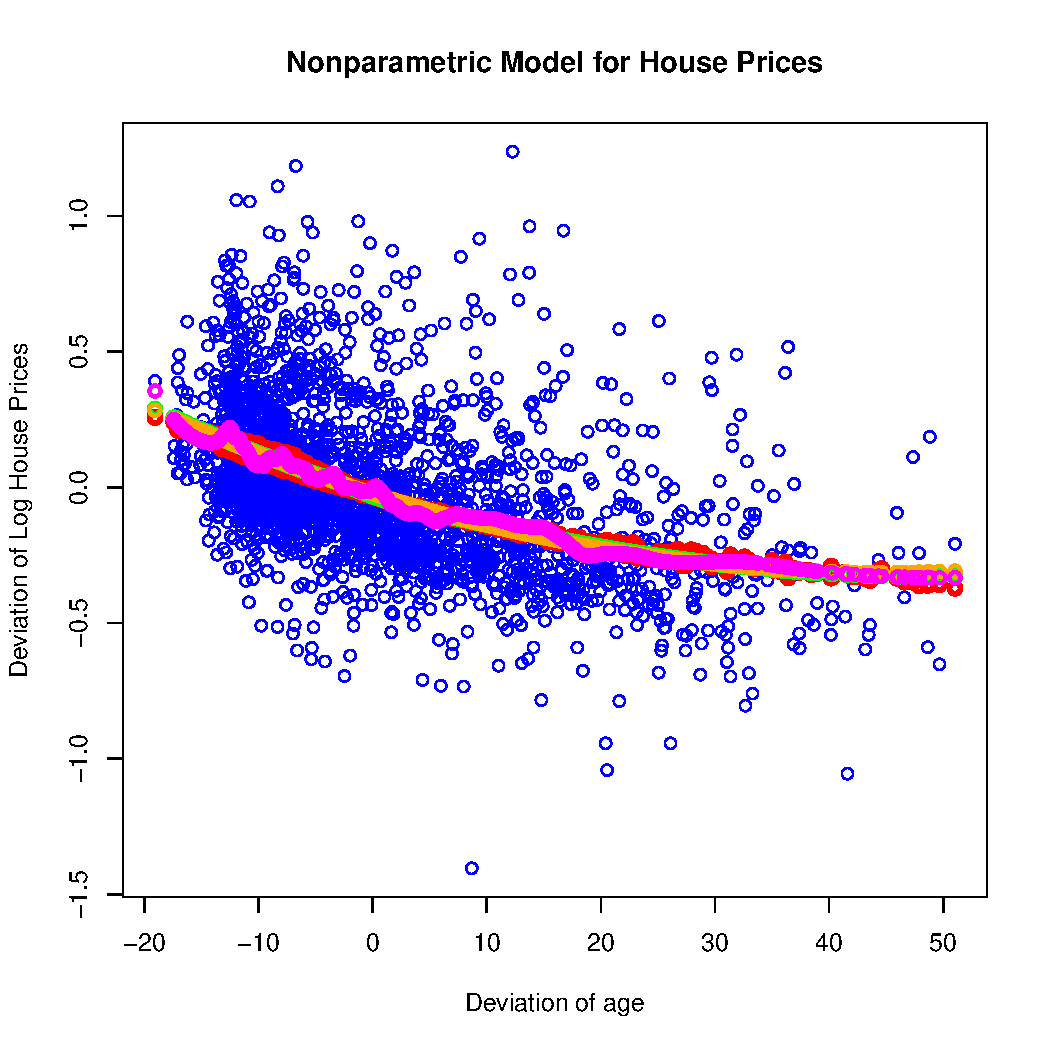
\includegraphics[scale = 0.5, keepaspectratio=true]{../Figures/dev_np_vs_age_dev_bw}
  \caption{Nonparametric Model for House Prices: Excess Age} \label{fig:dev_np_vs_age_dev_bw}
\end{figure}





\clearpage
\subsection{Nonparametric Specification for Lot Size}

As above, first conduct FWL regressions 
to reduce the problem to two dimensions. 
The models shown in
Table \ref{tab:reg_lot_fwl}
illustrate this possibility. 
Model 1 is the same original model in 
Table \ref{tab:reg_bt_age}. 
Model 2 is a regression omitting the age variable. 
Model 3 is a regression to predict age with the other explanatory variables in Model 2.
Finally, Model 4 shows the coefficient for Lot Size
from a regression of the residuals of Model 2
on the residuals from Model 3. 
Notice that these coefficients match those in Model 1. 


\begin{table}
\begin{center}
\begin{tabular}{l c c c c}
\hline
 & Original (1) & Reduced (2) & Lot Size (3) & FWL Lot Size (4) \\
\hline
(Intercept)       & $12.27956^{***}$ & $12.44426^{***}$ & $4570.55206^{***}$ &                 \\
                  & $(0.03468)$      & $(0.03096)$      & $(167.25090)$      &                 \\
TypeOfBuyerRental & $0.11437^{***}$  & $0.11974^{***}$  & $149.03169$        &                 \\
                  & $(0.01590)$      & $(0.01620)$      & $(87.51196)$       &                 \\
Age               & $-0.03428^{***}$ & $-0.03419^{***}$ & $2.63919$          &                 \\
                  & $(0.00365)$      & $(0.00372)$      & $(20.08503)$       &                 \\
NumBeds2          & $0.22090^{***}$  & $0.24652^{***}$  & $710.95724^{***}$  &                 \\
                  & $(0.02576)$      & $(0.02612)$      & $(141.13962)$      &                 \\
NumBeds3          & $0.41973^{***}$  & $0.47092^{***}$  & $1420.43656^{***}$ &                 \\
                  & $(0.03114)$      & $(0.03130)$      & $(169.09693)$      &                 \\
NumBeds4          & $0.60678^{***}$  & $0.64996^{***}$  & $1198.24876^{***}$ &                 \\
                  & $(0.03437)$      & $(0.03474)$      & $(187.71630)$      &                 \\
NumBeds6          & $0.69817^{***}$  & $0.81335^{***}$  & $3196.23145^{***}$ &                 \\
                  & $(0.05573)$      & $(0.05554)$      & $(300.08751)$      &                 \\
NumBeds8          & $1.07728^{***}$  & $1.22677^{***}$  & $4148.38835^{***}$ &                 \\
                  & $(0.06068)$      & $(0.05988)$      & $(323.52286)$      &                 \\
NumBaths2         & $0.07219^{***}$  & $0.08268^{***}$  & $290.99344^{***}$  &                 \\
                  & $(0.01376)$      & $(0.01398)$      & $(75.52624)$       &                 \\
NumBaths3         & $0.10791^{***}$  & $0.13008^{***}$  & $615.14719^{***}$  &                 \\
                  & $(0.02694)$      & $(0.02736)$      & $(147.81970)$      &                 \\
LotSize           & $0.00004^{***}$  &                  &                    &                 \\
                  & $(0.00000)$      &                  &                    &                 \\
HasGarage         & $0.26785^{***}$  & $0.34042^{***}$  & $2013.74849^{***}$ &                 \\
                  & $(0.01924)$      & $(0.01811)$      & $(97.84161)$       &                 \\
HasSecGate        & $0.22254^{***}$  & $0.22604^{***}$  & $97.24706$         &                 \\
                  & $(0.01788)$      & $(0.01822)$      & $(98.42853)$       &                 \\
TransitScore      & $0.06332^{***}$  & $0.05810^{***}$  & $-144.94653^{***}$ &                 \\
                  & $(0.00296)$      & $(0.00297)$      & $(16.03592)$       &                 \\
bt\_age\_log\_age & $0.00608^{***}$  & $0.00604^{***}$  & $-1.07046$         &                 \\
                  & $(0.00094)$      & $(0.00096)$      & $(5.17886)$        &                 \\
lot\_resid        &                  &                  &                    & $0.00004^{***}$ \\
                  &                  &                  &                    & $(0.00000)$     \\
\hline
R$^2$             & $0.67999$        & $0.66738$        & $0.56131$          & $0.03791$       \\
Adj. R$^2$        & $0.67817$        & $0.66562$        & $0.55899$          & $0.03752$       \\
Num. obs.         & $2473$           & $2473$           & $2473$             & $2473$          \\
\hline
\multicolumn{5}{l}{\scriptsize{$^{***}p<0.001$; $^{**}p<0.01$; $^{*}p<0.05$}}
\end{tabular}
\caption{Linear Model for Lot Size: FWL Regressions}
\label{tab:reg_lot_fwl}
\end{center}
\end{table}


\pagebreak 
To illustrate the fit of the model, 
Figure \ref{fig:dev_vs_lot} shows a scatter plot 
of the residual log prices on Lot Size. 
The observations are shown in blue
and the fitted values are shown in red.
The variation in the fitted values results from the 
fact that it is not plotted against the transformed excess lot size variable used in the regressions.
Still, the linear pattern is apparent
and appears to match the data. 

\begin{figure}[h!]
  \centering
  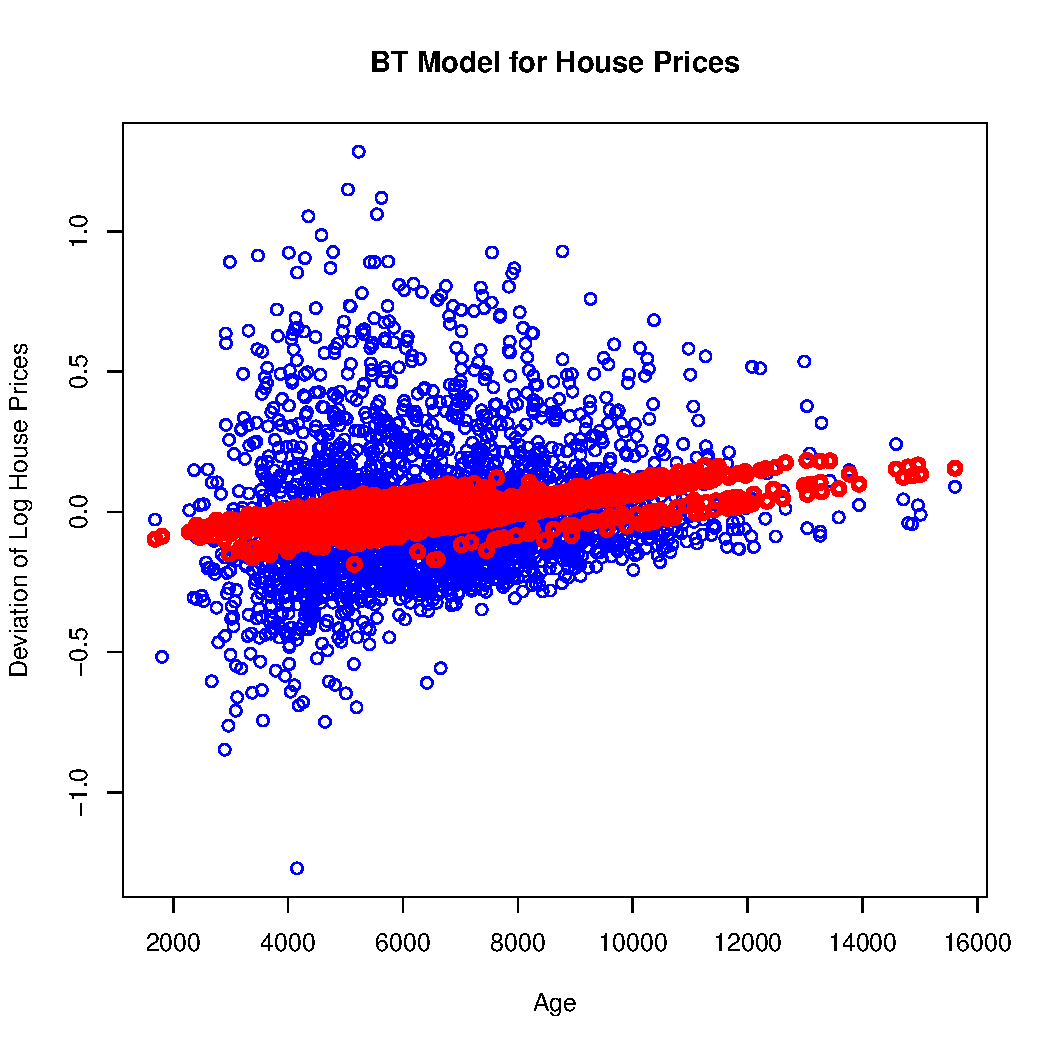
\includegraphics[scale = 0.5, keepaspectratio=true]{../Figures/dev_vs_lot}
  \caption{Linear-BT Model for House Prices} \label{fig:dev_vs_lot}
\end{figure}



\pagebreak
As a comparison, Figure \ref{fig:dev_vs_lot_dev} 
augments the above by showing the plot against the 
residuals from the regression for lot size:
the ``excess lot size'' of a house compared to what would be 
expected given the other characteristics of the hosue. 


\begin{figure}[h!]
  \centering
  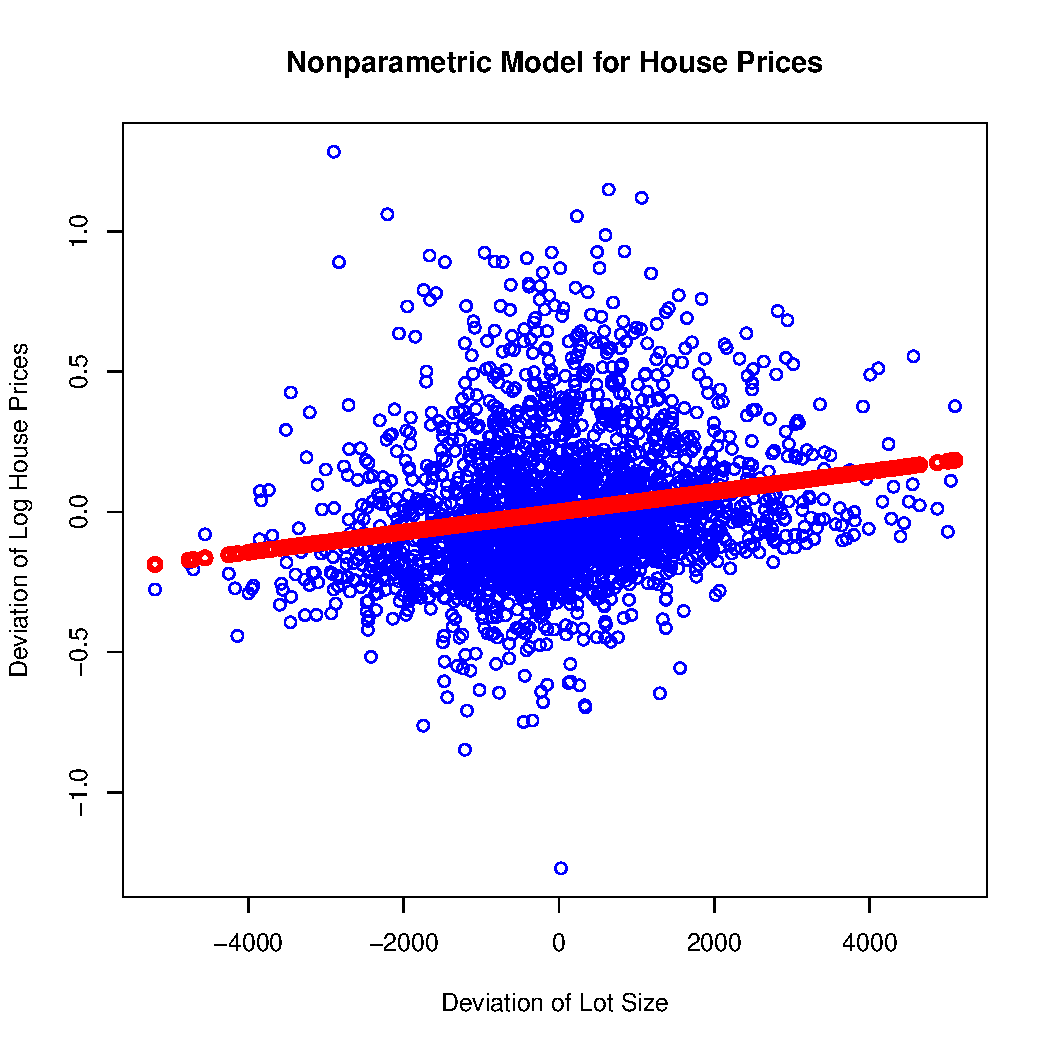
\includegraphics[scale = 0.5, keepaspectratio=true]{../Figures/dev_vs_lot_dev}
  \caption{Linear-BT Model for House Prices: Excess Lot Size} \label{fig:dev_vs_lot_dev}
\end{figure}

\clearpage
Now consider a nonparametric specification for 
the relationship between prices and Lot Size.
Figure \ref{fig:dev_np_vs_lot_dev} 
overlays the nonparametric estimate (shown in green) with the above in 
Figure \ref{fig:dev_vs_lot_dev}.
The pattern has more variation in slope but 
closely follows the prediction from the linear model. 
Although the nonparametric estimate varies around the linear estimate,
it appears that the linear form
is a close enough approximation without the added complexity.
Next, I will explore the transit score variable.


\begin{figure}[h!]
  \centering
  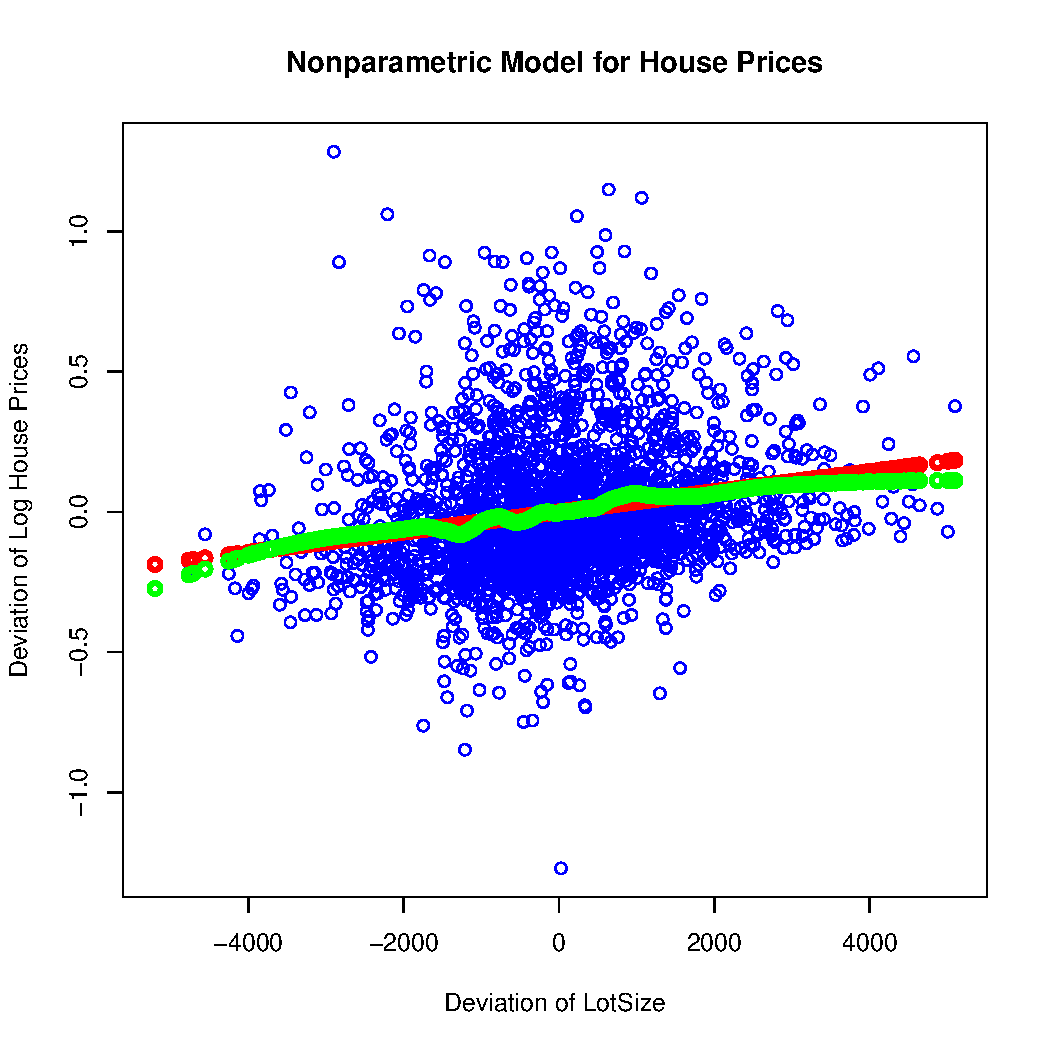
\includegraphics[scale = 0.5, keepaspectratio=true]{../Figures/dev_np_vs_lot_dev}
  \caption{Nonparametric Model for House Prices: Excess Lot Size} \label{fig:dev_np_vs_lot_dev}
\end{figure}





\clearpage
\subsection{Nonparametric Specification for Transit Score}

As above, first conduct FWL regressions 
to reduce the problem to two dimensions. 
The models shown in
Table \ref{tab:reg_trans_fwl}
illustrate this possibility. 
Model 1 is the same original model in 
Table \ref{tab:reg_bt_age}. 
Model 2 is a regression omitting the transit score variable. 
Model 3 is a regression to predict transit score with the other explanatory variables in Model 2.
Finally, Model 4 shows the coefficient for trasnit score
from a regression of the residuals of Model 2
on the residuals from Model 3. 
Notice that these coefficients match those in Model 1. 


\begin{table}
\begin{center}
\begin{tabular}{l c c c c}
\hline
 & Original (1) & Reduced (2) & Transit. (3) & FWL Transit (4) \\
\hline
(Intercept)       & $12.27956^{***}$ & $12.63639^{***}$ & $3.30691^{***}$  &                 \\
                  & $(0.03468)$      & $(0.03156)$      & $(0.19943)$      &                 \\
TypeOfBuyerRental & $0.11437^{***}$  & $0.16789^{***}$  & $0.82865^{***}$  &                 \\
                  & $(0.01590)$      & $(0.01721)$      & $(0.10875)$      &                 \\
Age               & $-0.03428^{***}$ & $-0.03571^{***}$ & $-0.02614$       &                 \\
                  & $(0.00365)$      & $(0.00399)$      & $(0.02525)$      &                 \\
NumBeds2          & $0.22090^{***}$  & $0.38493^{***}$  & $2.38241^{***}$  &                 \\
                  & $(0.02576)$      & $(0.02703)$      & $(0.17083)$      &                 \\
NumBeds3          & $0.41973^{***}$  & $0.68120^{***}$  & $3.61940^{***}$  &                 \\
                  & $(0.03114)$      & $(0.03160)$      & $(0.19969)$      &                 \\
NumBeds4          & $0.60678^{***}$  & $0.55368^{***}$  & $-1.65707^{***}$ &                 \\
                  & $(0.03437)$      & $(0.03697)$      & $(0.23364)$      &                 \\
NumBeds6          & $0.69817^{***}$  & $0.69526^{***}$  & $-2.03272^{***}$ &                 \\
                  & $(0.05573)$      & $(0.05935)$      & $(0.37507)$      &                 \\
NumBeds8          & $1.07728^{***}$  & $1.09572^{***}$  & $-2.25567^{***}$ &                 \\
                  & $(0.06068)$      & $(0.06396)$      & $(0.40421)$      &                 \\
NumBaths2         & $0.07219^{***}$  & $0.08315^{***}$  & $0.00810$        &                 \\
                  & $(0.01376)$      & $(0.01503)$      & $(0.09496)$      &                 \\
NumBaths3         & $0.10791^{***}$  & $0.12951^{***}$  & $-0.00978$       &                 \\
                  & $(0.02694)$      & $(0.02941)$      & $(0.18585)$      &                 \\
LotSize           & $0.00004^{***}$  &                  &                  &                 \\
                  & $(0.00000)$      &                  &                  &                 \\
HasGarage         & $0.26785^{***}$  & $0.34991^{***}$  & $0.16338$        &                 \\
                  & $(0.01924)$      & $(0.01946)$      & $(0.12297)$      &                 \\
HasSecGate        & $0.22254^{***}$  & $0.22158^{***}$  & $-0.07681$       &                 \\
                  & $(0.01788)$      & $(0.01958)$      & $(0.12374)$      &                 \\
TransitScore      & $0.06332^{***}$  &                  &                  &                 \\
                  & $(0.00296)$      &                  &                  &                 \\
bt\_age\_log\_age & $0.00608^{***}$  & $0.00634^{***}$  & $0.00507$        &                 \\
                  & $(0.00094)$      & $(0.00103)$      & $(0.00651)$      &                 \\
trans\_resid      &                  &                  &                  & $0.05810^{***}$ \\
                  &                  &                  &                  & $(0.00296)$     \\
\hline
R$^2$             & $0.67999$        & $0.61555$        & $0.62322$        & $0.13481$       \\
Adj. R$^2$        & $0.67817$        & $0.61368$        & $0.62138$        & $0.13446$       \\
Num. obs.         & $2473$           & $2473$           & $2473$           & $2473$          \\
\hline
\multicolumn{5}{l}{\scriptsize{$^{***}p<0.001$; $^{**}p<0.01$; $^{*}p<0.05$}}
\end{tabular}
\caption{Linear Model for Transit Score: FWL Regressions}
\label{tab:reg_trans_fwl}
\end{center}
\end{table}


\pagebreak 
To illustrate the fit of the model, 
Figure \ref{fig:dev_vs_trans} shows a scatter plot 
of the residual log prices on transit score. 
The observations are shown in blue
and the fitted values are shown in red.
The variation in the fitted values results from the 
fact that it is not plotted against the transformed excess transit score variable used in the regressions.
Still, the linear pattern is apparent
and appears to match the data. 

\begin{figure}[h!]
  \centering
  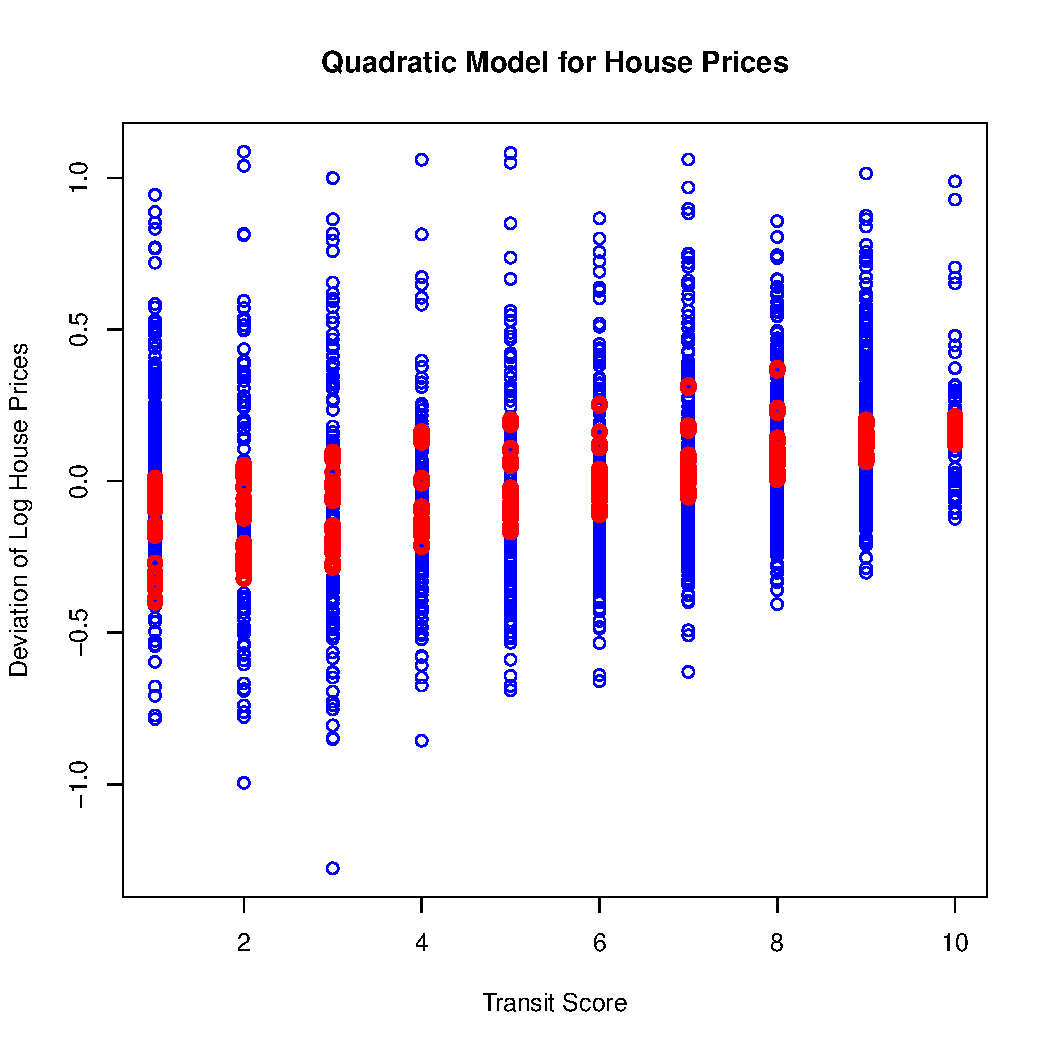
\includegraphics[scale = 0.5, keepaspectratio=true]{../Figures/dev_vs_trans}
  \caption{Linear-BT Model for House Prices} \label{fig:dev_vs_trans}
\end{figure}



\pagebreak
As a comparison, Figure \ref{fig:dev_np_vs_trans_dev} 
augments the above by showing the plot against the 
residuals from the regression for age:
the ``excess transit score'' of a house compared to what would be 
expected given the other characteristics of the house. 

% 
I move directly to the nonparametric specification for 
the relationship between prices and transit score.
Figure \ref{fig:dev_np_vs_trans_dev} 
overlays the nonparametric estimate, shown in green. 



\begin{figure}[h!]
  \centering
  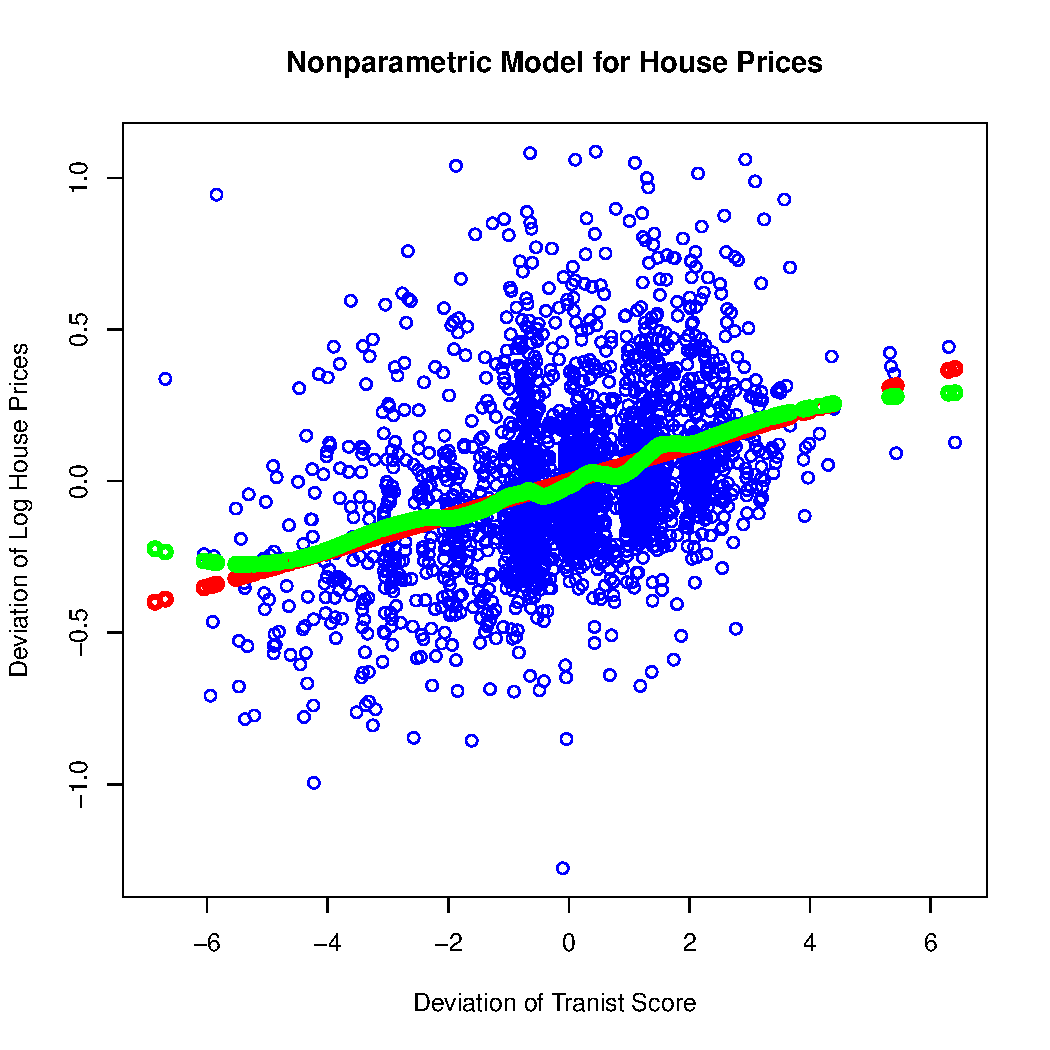
\includegraphics[scale = 0.5, keepaspectratio=true]{../Figures/dev_np_vs_trans_dev}
  \caption{Nonparametric Model for House Prices: Excess Transit Score} \label{fig:dev_np_vs_trans_dev}
\end{figure}

 

\pagebreak
\section{Semiparametric Estimates}

As I was building the above nonparametric models, 
I stored the predictions and will now use them as variables in 
linear models. 
Table \ref{tab:reg_semipar} 
shows the estimates from a set of models. 
Model 1 is the benchmark linear model in 
Table \ref{tab:reg_bt_age}. 
Model 2 is a semi-parametric model
with a nonparametric fit on age
substituted in for the age variables.
Models 3 and 4 are semi-parametric models
with nonparametric fits on lot size and transit score, respectively.
Model 5 is a maximally semiparametric model, 
with nonparametric fits for all continuous variables. 
For each of the single-variable semiparametric models, 
the coefficients are near one
and the fits are similar to the linear model. 
Even with maximal flexibility, the fit of Model 5
is not much better than the benchmark linear model. 
Across models 1, 4 and 5, the adjusted $\bar{R}^2$ values are all hovering around 0.62. 
All things considered, these are excellent models
and the linear model is sufficient.


\begin{table}
\begin{center}
\begin{tabular}{l c c c c c}
\hline
 & Model 1 & Model 2 & Model 3 & Model 4 & Model 5 \\
\hline
(Intercept)       & $12.27956^{***}$ & $12.46848^{***}$ & $12.63542^{***}$ & $12.63901^{***}$ & $12.47247^{***}$ \\
                  & $(0.03468)$      & $(0.02944)$      & $(0.03100)$      & $(0.02928)$      & $(0.02643)$      \\
TypeOfBuyerRental & $0.11437^{***}$  & $0.09463^{***}$  & $0.16816^{***}$  & $0.16510^{***}$  & $0.09156^{***}$  \\
                  & $(0.01590)$      & $(0.01725)$      & $(0.01690)$      & $(0.01597)$      & $(0.01549)$      \\
Age               & $-0.03428^{***}$ &                  & $-0.03531^{***}$ & $-0.03555^{***}$ &                  \\
                  & $(0.00365)$      &                  & $(0.00392)$      & $(0.00371)$      &                  \\
NumBeds2          & $0.22090^{***}$  & $0.39266^{***}$  & $0.38449^{***}$  & $0.37968^{***}$  & $0.38653^{***}$  \\
                  & $(0.02576)$      & $(0.02737)$      & $(0.02655)$      & $(0.02508)$      & $(0.02457)$      \\
NumBeds3          & $0.41973^{***}$  & $0.69266^{***}$  & $0.68003^{***}$  & $0.67808^{***}$  & $0.68809^{***}$  \\
                  & $(0.03114)$      & $(0.03200)$      & $(0.03104)$      & $(0.02932)$      & $(0.02872)$      \\
NumBeds4          & $0.60678^{***}$  & $0.55581^{***}$  & $0.55357^{***}$  & $0.54859^{***}$  & $0.55004^{***}$  \\
                  & $(0.03437)$      & $(0.03744)$      & $(0.03632)$      & $(0.03430)$      & $(0.03361)$      \\
NumBeds6          & $0.69817^{***}$  & $0.70465^{***}$  & $0.69855^{***}$  & $0.71472^{***}$  & $0.72890^{***}$  \\
                  & $(0.05573)$      & $(0.06010)$      & $(0.05830)$      & $(0.05507)$      & $(0.05396)$      \\
NumBeds8          & $1.07728^{***}$  & $1.15277^{***}$  & $1.10040^{***}$  & $1.10802^{***}$  & $1.17134^{***}$  \\
                  & $(0.06068)$      & $(0.06475)$      & $(0.06283)$      & $(0.05934)$      & $(0.05813)$      \\
NumBaths2         & $0.07219^{***}$  & $0.08847^{***}$  & $0.08286^{***}$  & $0.08323^{***}$  & $0.08830^{***}$  \\
                  & $(0.01376)$      & $(0.01522)$      & $(0.01476)$      & $(0.01394)$      & $(0.01366)$      \\
NumBaths3         & $0.10791^{***}$  & $0.13918^{***}$  & $0.12915^{***}$  & $0.12929^{***}$  & $0.13893^{***}$  \\
                  & $(0.02694)$      & $(0.02977)$      & $(0.02889)$      & $(0.02728)$      & $(0.02672)$      \\
LotSize           & $0.00004^{***}$  &                  &                  &                  &                  \\
                  & $(0.00000)$      &                  &                  &                  &                  \\
HasGarage         & $0.26785^{***}$  & $0.29027^{***}$  & $0.35095^{***}$  & $0.34982^{***}$  & $0.29112^{***}$  \\
                  & $(0.01924)$      & $(0.01959)$      & $(0.01912)$      & $(0.01805)$      & $(0.01759)$      \\
HasSecGate        & $0.22254^{***}$  & $0.18970^{***}$  & $0.22175^{***}$  & $0.22100^{***}$  & $0.18897^{***}$  \\
                  & $(0.01788)$      & $(0.01980)$      & $(0.01923)$      & $(0.01817)$      & $(0.01777)$      \\
TransitScore      & $0.06332^{***}$  &                  &                  &                  &                  \\
                  & $(0.00296)$      &                  &                  &                  &                  \\
bt\_age\_log\_age & $0.00608^{***}$  &                  & $0.00623^{***}$  & $0.00630^{***}$  &                  \\
                  & $(0.00094)$      &                  & $(0.00101)$      & $(0.00096)$      &                  \\
age\_np           &                  & $0.98989^{***}$  &                  &                  & $1.03645^{***}$  \\
                  &                  & $(0.04111)$      &                  &                  & $(0.03695)$      \\
lot\_np           &                  &                  & $1.00375^{***}$  &                  & $1.06134^{***}$  \\
                  &                  &                  & $(0.10570)$      &                  & $(0.09782)$      \\
trans\_np         &                  &                  &                  & $1.02370^{***}$  & $1.10299^{***}$  \\
                  &                  &                  &                  & $(0.05125)$      & $(0.05028)$      \\
\hline
R$^2$             & $0.67999$        & $0.60556$        & $0.62915$        & $0.66923$        & $0.68242$        \\
Adj. R$^2$        & $0.67817$        & $0.60380$        & $0.62719$        & $0.66748$        & $0.68074$        \\
Num. obs.         & $2473$           & $2473$           & $2473$           & $2473$           & $2473$           \\
\hline
\multicolumn{6}{l}{\scriptsize{$^{***}p<0.001$; $^{**}p<0.01$; $^{*}p<0.05$}}
\end{tabular}
\caption{Semiparametric Models for House Prices}
\label{tab:reg_semipar}
\end{center}
\end{table}






\pagebreak
\section{Generalized Additive Model}

\subsection{Linear Model}

As an example of the output from the GAM specification, 
I first estimated the model with no nonlinear terms, 
which is essentially a linear regression. 

\begin{verbatim}
Family: gaussian 
Link function: identity 

Formula:
log_Price ~ TypeOfBuyer + NumBeds + NumBaths + HasGarage + HasSecGate + 
    bt_age_log_age + Age

Parametric coefficients:
                   Estimate Std. Error t value Pr(>|t|)    
(Intercept)       12.636387   0.031557 400.428  < 2e-16 ***
TypeOfBuyerRental  0.167885   0.017208   9.756  < 2e-16 ***
NumBeds2           0.384933   0.027031  14.240  < 2e-16 ***
NumBeds3           0.681198   0.031598  21.559  < 2e-16 ***
NumBeds4           0.553684   0.036969  14.977  < 2e-16 ***
NumBeds6           0.695256   0.059348  11.715  < 2e-16 ***
NumBeds8           1.095722   0.063960  17.131  < 2e-16 ***
NumBaths2          0.083150   0.015026   5.534 3.46e-08 ***
NumBaths3          0.129513   0.029408   4.404 1.11e-05 ***
HasGarage          0.349911   0.019458  17.983  < 2e-16 ***
HasSecGate         0.221579   0.019581  11.316  < 2e-16 ***
bt_age_log_age     0.006339   0.001030   6.153 8.86e-10 ***
Age               -0.035709   0.003995  -8.938  < 2e-16 ***
---
Signif. codes:  0 �***� 0.001 �**� 0.01 �*� 0.05 �.� 0.1 � � 1


R-sq.(adj) =  0.614   Deviance explained = 61.6%
GCV = 0.077393  Scale est. = 0.076987  n = 2473
\end{verbatim}

\pagebreak
\subsection{Semiparametric Model}


Further investigating the results of the full semiparametric specification
of Model 5 of Table \ref{tab:reg_semipar},
I estimated the model with all three continuous variables specified as nonparametric functions. 
The result was that 
almost all the variables---both linear and nonlinear---were 
statistically significant. 


\begin{verbatim}
Family: gaussian 
Link function: identity 

Formula:
log_Price ~ s(Age) + s(LotSize) + s(TransitScore) + TypeOfBuyer + 
    NumBeds + NumBaths + HasGarage + HasSecGate

Parametric coefficients:
                  Estimate Std. Error t value Pr(>|t|)    
(Intercept)       12.66687    0.03019 419.567  < 2e-16 ***
TypeOfBuyerRental  0.11042    0.01605   6.880 7.59e-12 ***
NumBeds2           0.21419    0.02606   8.218 3.31e-16 ***
NumBeds3           0.40513    0.03149  12.865  < 2e-16 ***
NumBeds4           0.58441    0.03644  16.037  < 2e-16 ***
NumBeds6           0.69712    0.05784  12.053  < 2e-16 ***
NumBeds8           1.08605    0.06412  16.938  < 2e-16 ***
NumBaths2          0.07120    0.01373   5.186 2.32e-07 ***
NumBaths3          0.10819    0.02686   4.027 5.81e-05 ***
HasGarage          0.25377    0.01974  12.856  < 2e-16 ***
HasSecGate         0.22450    0.01785  12.576  < 2e-16 ***
---
Signif. codes:  0 �***� 0.001 �**� 0.01 �*� 0.05 �.� 0.1 � � 1

Approximate significance of smooth terms:
                  edf Ref.df      F p-value    
s(Age)          2.893  3.614 201.80  <2e-16 ***
s(LotSize)      3.127  4.010  27.57  <2e-16 ***
s(TransitScore) 2.989  3.756 126.22  <2e-16 ***
---
Signif. codes:  0 �***� 0.001 �**� 0.01 �*� 0.05 �.� 0.1 � � 1

R-sq.(adj) =   0.68   Deviance explained = 68.3%
GCV = 0.06425  Scale est. = 0.063731  n = 2473
\end{verbatim}

On the other hand, 
the adjusted R-squared has decreased
from 0.68 to 0.614 under this specification, 
which therefore suggests this complex model is not efficient as the more simpler one.


Perhaps as a middle ground, we can estimate a model with a 
nonparametric specification for the age variable alone, 
since it seems to have a nonlinear relationship with value in either case. 
This retains most of the predictive value of the maximally 
semiparametric model and accommodates the 
nonlinear relationship with value of age. This brought the adjusted R Squared back up to .68 but still the model is too complex to be chosen and the original model chosen in Problem Set 7 should be used.

\begin{verbatim}
Family: gaussian 
Link function: identity 

Formula:
log_Price ~ s(Age) + LotSize + TransitScore + TypeOfBuyer + NumBeds + 
    NumBaths + HasGarage + HasSecGate

Parametric coefficients:
                   Estimate Std. Error t value Pr(>|t|)    
(Intercept)       1.206e+01  3.275e-02 368.273  < 2e-16 ***
LotSize           3.606e-05  3.665e-06   9.839  < 2e-16 ***
TransitScore      6.339e-02  2.963e-03  21.397  < 2e-16 ***
TypeOfBuyerRental 1.145e-01  1.592e-02   7.195 8.24e-13 ***
NumBeds2          2.201e-01  2.578e-02   8.535  < 2e-16 ***
NumBeds3          4.191e-01  3.117e-02  13.447  < 2e-16 ***
NumBeds4          6.070e-01  3.440e-02  17.648  < 2e-16 ***
NumBeds6          6.992e-01  5.579e-02  12.532  < 2e-16 ***
NumBeds8          1.076e+00  6.073e-02  17.720  < 2e-16 ***
NumBaths2         7.248e-02  1.377e-02   5.264 1.53e-07 ***
NumBaths3         1.078e-01  2.696e-02   3.997 6.59e-05 ***
HasGarage         2.675e-01  1.925e-02  13.895  < 2e-16 ***
HasSecGate        2.226e-01  1.789e-02  12.441  < 2e-16 ***
---
Signif. codes:  0 �***� 0.001 �**� 0.01 �*� 0.05 �.� 0.1 � � 1

Approximate significance of smooth terms:
         edf Ref.df     F p-value    
s(Age) 2.908  3.632 198.3  <2e-16 ***
---
Signif. codes:  0 �***� 0.001 �**� 0.01 �*� 0.05 �.� 0.1 � � 1

R-sq.(adj) =  0.678   Deviance explained =   68%
GCV = 0.064646  Scale est. = 0.06423   n = 2473
\end{verbatim}



%%%%%%%%%%%%%%%%%%%%%%%%%%%%%%%%%%%%%%%%
%\end{document}
%%%%%%%%%%%%%%%%%%%%%%%%%%%%%%%%%%%%%%%%
